% !TEX root = ../TSG_Administrator's_Guide_Latest_EN.tex
%
\pdfbookmark[0]{Appendix E TSG Packet Flow}{Appendix E TSG Packet Flow}
\chapter*{\hypertarget{link:Appendix E TSG Packet Flow}{Appendix E TSG Packet Flow}}
\label{sec:appendix_e}

\pdfbookmark[1]{Overview}{Overview}
\section*{\hypertarget{link:Overview}{Overview}}
\label{sec:appendix_e:overview}

This document describes the packet handling sequence in TSG. TSG Firewall performs stateful checks, TSG proxy performs decryption. 


The Ingress stage, session stage and egress stage are the three stages of TSG traffic processing. The ingress and egress stages handle network functions and make packet forwarding decisions on a per-packet basis. The remaining stages are session-based security functions such as application identification and content inspection. TSG does not change the operation of the MPLS, 802.1Q, IPv4, IPv6 protocols regardless of the configured policies.

%\begin{figure}[htb]
	%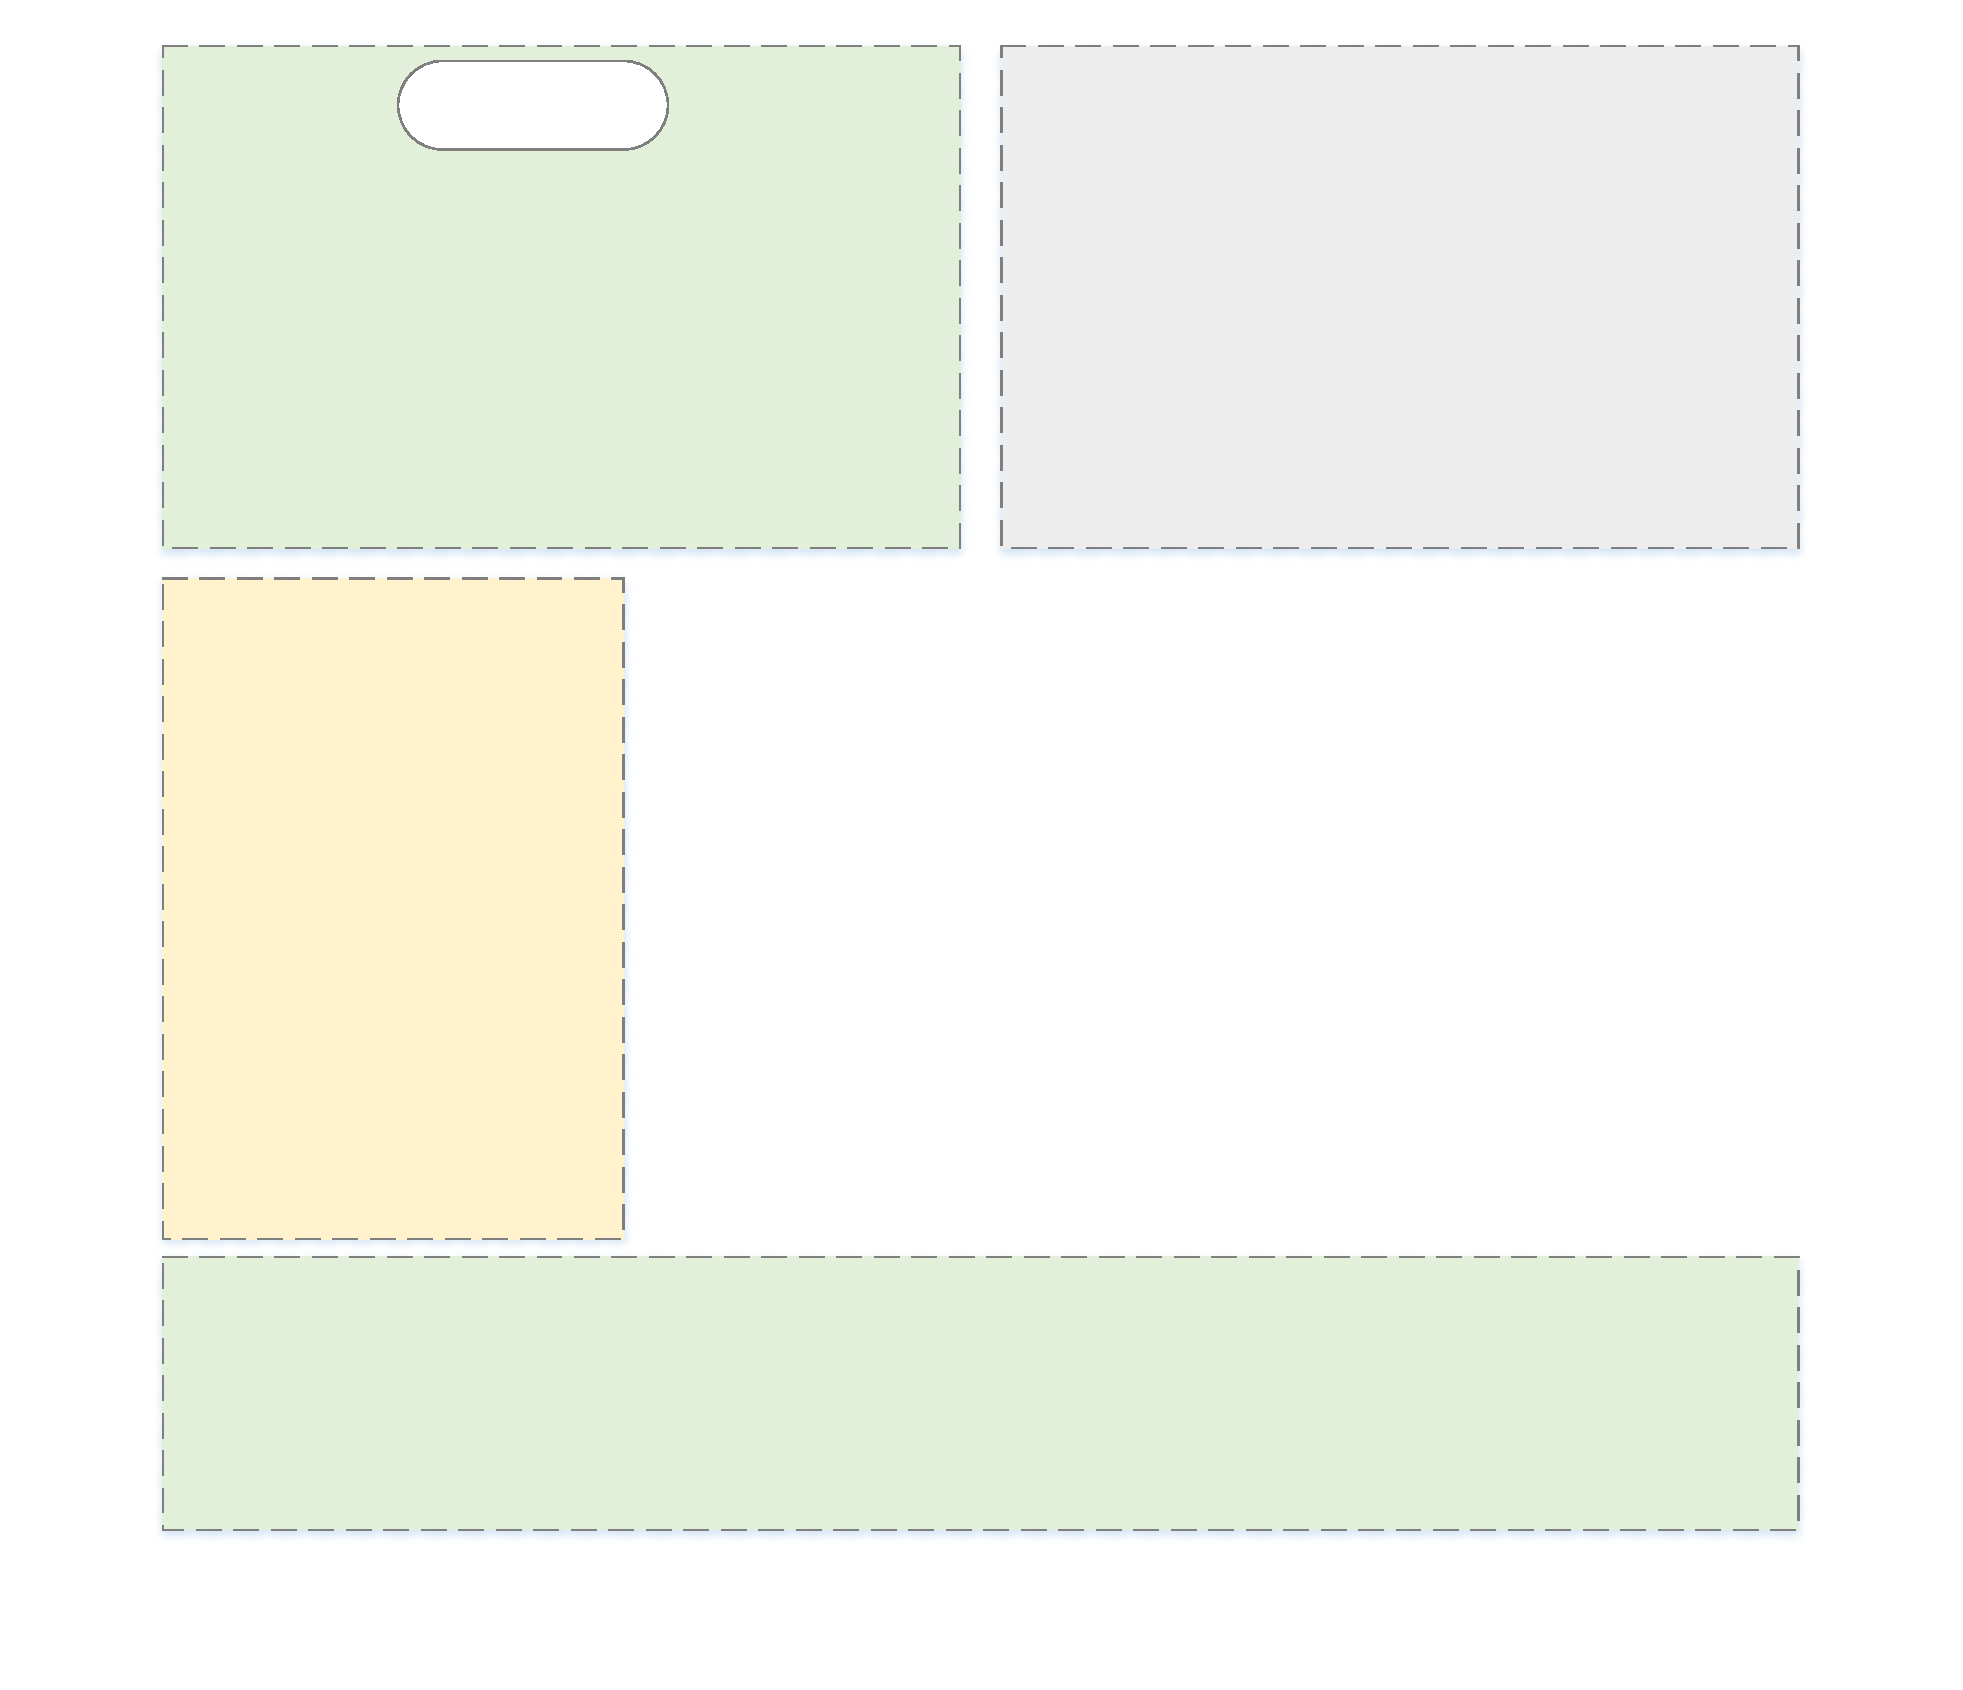
\includegraphics[width=\textwidth]{images/pakcet_life_2020}
	%\caption{Figure: Inspection Stage}
	%\label{fig:system:pakcet_life_2020}
%\end{figure}

\begin{figure}
    \centering
    \includesvg{1.6\columnwidth}{../images/pakcet_life_2020}
    %\caption{Figure}
\end{figure}

\pdfbookmark[1]{Packet Handling Sequence}{Packet Handling Sequence}
\section*{\hypertarget{link:Packet Handling Sequence}{Packet Handling Sequence}}
\label{sec:appendix_e:sequence}

\pdfbookmark[2]{Ingress stage}{Ingress stage}
\subsection*{\hypertarget{link:Ingress stage}{Ingress stage}}
\label{sec:appendix_e:sequence:ingress}

The ingress stage receives packets from the network interface, parses those packets, and then determines whether a given packet is subject to further inspection. If the packet is subject to further inspection, the system continues with a session lookup and the packet enters the session stage. Otherwise, the system forwards the packet to the egress stage.

\pdfbookmark[3]{Layer 2 Decode}{Layer 2 Decode}
\subsubsection*{\hypertarget{link:Layer 2 Decode}{Layer 2 Decode}}
\label{sec:appendix_e:sequence:ingress:decode}

Packet parsing starts with the Ethernet (Layer-2) header of the packet received from the wire. VLAN, MPLS, MAC\_IN\_MAC headers are parsed here. The ingress port, 802.1q tag, and destination MAC address are used as keys to lookup the ingress logical interface. 

\pdfbookmark[3]{Tunnel Decapsulation}{Tunnel Decapsulation}
\subsubsection*{\hypertarget{link:Tunnel Decapsulation}{Tunnel Decapsulation}}
\label{sec:appendix_e:sequence:ingress:decapsulation}

If the packet has PPPOE, IPIP, GRE, PPTP, L2TP, Teredo, GTP encapsulations, they are decoded at this stage.

\pdfbookmark[3]{IP Defragmentation}{IP Defragmentation}
\subsubsection*{\hypertarget{link:IP Defragmentation}{IP Defragmentation}}
\label{sec:appendix_e:sequence:ingress:defragmentation}

After the IP header is parsed (Layer-3), the TSG parses IP fragments, reassembles using the defragmentation process, and then feeds the packet back to the parser starting with the IP header.  At this stage, a fragment may be discarded due to tear-drop attack (overlapping fragments), fragmentation errors, or if the TSG hits system limits on buffered fragments (hits the max packet threshold).

\pdfbookmark[2]{Session Setup}{Session Setup}
\subsection*{\hypertarget{link:Session Setup}{Session Setup}}
\label{sec:appendix_e:sequence:setup}

If the packet is subject to firewall inspection, it performs a flow lookup on the packet. In TSG ’s implementation, the firewall identifies the flow using a 5-tuple key:


• Source and destination IP addresses: IP addresses from the IP packet. 


• Source and destination ports: Port numbers from TCP/UDP protocol headers. For non-TCP/UDP, different protocol fields are used (e.g., for ICMP the ICMP identifier and sequence numbers are used).


• Protocol: The IP protocol number from the IP header is used to derive the flow key. 


The firewall stores active flows in the flow lookup table. When a packet is determined to be eligible for firewall inspection, the firewall extracts the 5-tuple flow key from the packet and then performs a flow lookup to match the packet with an existing flow. Each flow has a client and server component. For TCP, the client is the sender of the TCP SYN packet of the session from firewall’s perspective. For UDP, the client is the sender with smaller Port number. The server is the receiver of this first packet. 


If the packet belongs to on new session, firewall performs a session setup.


The firewall uses the IP address of the packet to query mapping tables.


• Subscriber-IP mapping table: The corresponding user information is fetched.


• ASN-IP mapping table: The autonomous system number is fetched.


• Geo-IP mapping table: The geographical location is fetched.


There is a chance that above information is not available at this point. In that case, policies with these conditions cannot be enforced.

\pdfbookmark[2]{Session Maintenance}{Session Maintenance}
\subsection*{\hypertarget{link:Session Maintenance}{Session Maintenance}}
\label{sec:appendix_e:sequence:maintenance}

A packet that matches an existing session will enter the session maintenance stages. This stage starts with Layer 2 to Layer 4 firewall processing:


• If the session is in close wait state, then the firewall discards the packet by forwarding to egress stage. 


• If the session is active, refresh session timeout.


• If the packet is a TCP FIN/RST, the session TCP half closed timer is started if this is the first FIN packet received (half closed session) or the TCP Time Wait timer is started if this is the second FIN packet or RST packet. The session is closed as soon as either of these timers expire. 


If an application uses TCP as the transport, the firewall processes it by the TCP reassembly module before it sends the data stream into the security-processing module. The TCP reassembly module will also perform window check, buffer out-of-order data while skipping TCP retransmission. The firewall drops the packets if there is a reassembly error or if it receives too many out-of-order fragments, resulting in the reassembly buffers filling up.


A packet matching an existing session is subject to further processing if packet has TCP/UDP data (payload). If the firewall does not detect the session application, it performs application identification. If the identification is non-conclusive, the content inspection module runs known protocol decoder checks and heuristics to help identify the application. The application identification result could change throughout the life of the session. Once a traffic attribute is parsed, it’s subject to security policy enforcement.

\pdfbookmark[2]{Firewall Process}{Firewall Process}
\subsection*{\hypertarget{link:Firewall Process}{Firewall Process}}
\label{sec:appendix_e:sequence:firewall}

\pdfbookmark[3]{Layer 7 Decode}{Layer 7 Decode}
\subsubsection*{\hypertarget{link:Layer 7 Decode}{Layer 7 Decode}}
\label{sec:appendix_e:sequence:firewall:decode}

The firewall decodes Layer 7 protocols such as HTTP, SSL/TLS and DNS, to get traffic attributes.

\pdfbookmark[3]{Application Identification}{Application Identification}
\subsubsection*{\hypertarget{link:Application Identification}{Application Identification}}
\label{sec:appendix_e:sequence:firewall:identification}

The firewall identifies application with built-in and customized signature. The firewall uses protocol decoding in the content inspection stage to determine if an application changes from one application to another. After the firewall identifies the session application, security policy will be enforced as configured. 

\pdfbookmark[3]{Content Decode}{Content Decode}
\subsubsection*{\hypertarget{link:Content Decode}{Content Decode}}
\label{sec:appendix_e:sequence:firewall:contentdecode}

The firewall decodes the flow and parses attributes and content, then scan them for keywords, e.g., email attachments that are text-based. If it results in keywords detection, then the corresponding security policy action is taken. Application identification is still on at this stage, as the more traffic attributes are parsed, application identification result may be changed. 

\pdfbookmark[3]{Security Policy Lookup}{Security Policy Lookup}
\subsubsection*{\hypertarget{link:Security Policy Lookup}{Security Policy Lookup}}
\label{sec:appendix_e:sequence:firewall:lookup}

The firewall uses application ANY, IP, port, Geographic and Subscriber ID to perform the lookup and check for a rule match. In case of a rule match, if the policy action is set to ‘deny’, the firewall drops the packet. 


If security policy action is set to intercept and the application is SSL or HTTP, the firewall sends session packets to Proxy to perform decryption.


After more packet transferred, identified application as well as FQDN, URL and applicable protocol fields in the session are used as key to find rule match. If the session matches a security rule, and the rule has logging enabled, the firewall generates a security event log at the session end.

\pdfbookmark[2]{Proxy Process}{Proxy Process}
\subsection*{\hypertarget{link:Proxy Process}{Proxy Process}}
\label{sec:appendix_e:sequence:proxy}

\pdfbookmark[3]{Duplicate Packet Processing}{Duplicate Packet Processing}
\subsubsection*{\hypertarget{link:Duplicate Packet Processing}{Duplicate Packet Processing}}
\label{sec:appendix_e:sequence:proxy:duplicate}

Packet usually travels a route one time only, otherwise it’s a waste of bandwidth. But network of real world is complicated: tunnels, policy ACLs and human mistakes all induce packet travels a link more than one time.


This will cause problems on Proxy function. When Proxy terminates server-side SSL connections, as a client, it sends packet to server with original 4-tuple, and that packet goes through TSG again. Since this packet has the same 4-tuple and sequence number as the client-side, TSG will drop it as a client-side retransmission packet, which causes server-side timeout.


The proxy fixes this problem by following two mechanisms:


• Duplicate packet identification: For TSG sent packets, TSG adds its 4-tuple, IPID, acknowledge number, sequence number and timestamp (if applicable) to the Bloom filter. For received packet, TSG will query the Bloom filter with the aforementioned protocol fields. If a packet is considered duplicate, it will be bypassed, if not, it will be delivered to TCP stack.


• Duplicate flow detection: Since not all traffic flows have duplicate packets, do duplicate identification on each packet is a waste of CPU and memory, moreover, it induces performance overhead. Hence, only the TCP flows with duplicate SYN or SYN/ACK packet will conduct duplicate packet identification. 

\pdfbookmark[3]{TCP Stack}{TCP Stack}
\subsubsection*{\hypertarget{link:TCP Stack}{TCP Stack}}
\label{sec:appendix_e:sequence:proxy:TCP}

Opening a TCP connection involves a three-way handshake involving packets: the client contacts the server, the server acknowledges the client, and the client acknowledges the server. The proxy’s TCP stack attempts to connect server-side immediately after receiving the client's initial connection request, but waits to return the server acknowledgement until determining whether or not the server-side connection succeeds. This provides greater transparency, as the client receives either an RST or no response, which mirrors what is sent from a server when connections fail.

\pdfbookmark[3]{Build SSL Session}{Build SSL Session}
\subsubsection*{\hypertarget{link:Build SSL Session}{Build SSL Session}}
\label{sec:appendix_e:sequence:proxy:build}

The proxy first builds server-side SSL session, if the server certificate verification is failed, the proxy will sign certificate with untrusted root. That’s because the proxy wants the untrust certificate to warn users that they are trying to access potentially unsafe sites.

\pdfbookmark[3]{Proxy Policy Lookup}{Proxy Policy Lookup}
\subsubsection*{\hypertarget{link:Proxy Policy Lookup}{Proxy Policy Lookup}}
\label{sec:appendix_e:sequence:proxy:lookup}

After decode Layer 7 protocols, traffic attributes like HTTP URL, headers are subject to proxy policy lookup, then according action is taken.

\pdfbookmark[3]{Re-encryption}{Re-encryption}
\subsubsection*{\hypertarget{link:Re-encryption}{Re-encryption}}
\label{sec:appendix_e:sequence:proxy:re-encryption}

The content is compressed and encrypted, and send to egress stage

\pdfbookmark[2]{Egress Stage}{Egress Stage}
\subsection*{\hypertarget{link:Egress Stage}{Egress Stage}}
\label{sec:appendix_e:sequence:egress}

The system identifies encapsulation information for the packet, including MAC addresses, VLAN ID and tunnel headers. And find the egress interface.
Finally, the packet is transmitted out of the physical egress interface.
